%
% File acl2015.tex
%
% Contact: yanglinfang@berkeley.edu
%%
%% Based on the style files for ACL-2014, which were, in turn,
%% Based on the style files for ACL-2013, which were, in turn,
%% Based on the style files for ACL-2012, which were, in turn,
%% based on the style files for ACL-2011, which were, in turn, 
%% based on the style files for ACL-2010, which were, in turn, 
%% based on the style files for ACL-IJCNLP-2009, which were, in turn,
%% based on the style files for EACL-2009 and IJCNLP-2008...

%% Based on the style files for EACL 2006 by 
%%e.agirre@ehu.es or Sergi.Balari@uab.es
%% and that of ACL 08 by Joakim Nivre and Noah Smith

\documentclass[11pt]{article}
\usepackage{acl2015}
\usepackage{times}
\usepackage{url}
\usepackage{latexsym}
\usepackage{graphicx}

%\setlength\titlebox{5cm}

% You can expand the titlebox if you need extra space
% to show all the authors. Please do not make the titlebox
% smaller than 5cm (the original size); we will check this
% in the camera-ready version and ask you to change it back.


\title{Scalable Low Quality News Identification}

\author{Linfang Yang \\
  UC Berkeley / MIDS W266 Monday\\
  {\tt yanglinfang@berkeley.edu} \\\And
  Ricardo Barrera \\
  UC Berkeley / MIDS W266 Monday \\
  {\tt ricardofrank@berkeley.edu} \\}

\date{\today}

\begin{document}
\maketitle
\begin{abstract}
Convolutional Neural Networks (CNNs) greatly improve modeling sophistication and power which enables certain scenarios in Natural Language Processing such as document classification and feature extraction to perform adequately for consumer use.  In this paper, we discuss leveraging existing work using CNNs to rate articles along fourteen dimensions of labels describing article quality (e.g. 'Conciseness') and explore the possible connection between article veracity and quality via correlations.  The motivation for this effort stems from the exponential growth in media that will further exacerbate the problem of misinformation overload.
\end{abstract}

\section{Introduction and Background}

\indent \indent Modern society suffers from an overwhelming amount of information due to technological advancements that make incessant and ubiquitous media consumption the norm.  As a result, consumers now have a uniquely modern challenge to filter and validate their information sources to avoid misleading information, which we call 'Low Quality News'.  \\
\indent Unfortunately, it is unreasonable to expect individuals to filter and verify all of the incoming information.  This presents and opportunity to assist individuals by automatically labeling content to quickly and easily to identify low quality information, similar to but not entirely described by the colloquial term, 'Fake News'. \\
\indent This project leverages existing work to classify articles via Convolutional Neural Networks (CNNs) based upon fourteen different dimensions (e.g. 'Comprehensiveness' and 'Conciseness') in an ensemble fashion to identify low-quality news articles. \textit{[6]} The long-term vision is to eventually create a news categorization platform that will allow people to filter and curate their content quickly, easily, and reliably. \\
\indent The evaluation and exploration process involved gathering many Facebook articles that were already labeled as a part of a BuzzFeed article dataset examining the quality of major information sources on Facebook, with the goal of being able to identify correlations between article quality and article veracity, identified with the categories: 'Mostly True', 'Mix of True and False', 'Mostly False', and 'No Factual Content'. \textit{[5]}  

\section{Datasets Selection Process}

\indent \indent There are very few datasets publicly available online with labeling for article quality and veracity, and generating new datasets is expensive and time consuming.  Therefore, we worked with whatever datasets we could find.  If the effort showed promise, it would then prove worthwhile to fund and generate a new dataset in-house and further investigate.

\subsection{Fake News Kaggle Dataset}
\url{https://www.kaggle.com/mrisdal/fake-news} \\

\indent \indent We did not end up using this dataset in our final results for various reasons, but it is worth exploring later since it provides automatically labeled data, which can be useful to evaluate a more mature system later on. It contains text and metadata from 244 websites and represents 12999 posts in total from the past 30 years, pulled using webhouse.io API. Then it used BS Detector to label the dataset as fake or not. We found that the dataset is heavily skewed towards not fake. It is understandable that there are less fake news than actual news on the web. We preferred using dataset generated by human rather than by another labeling system so that we did not inherit bias in the BS Detector.  

\subsection{Yahoo News Quality Dataset}
\url{http://novasearch.org/datasets/} \\

This dataset is from NOVE Search . It contains 500 news articles and manual labels from professional linguist or editor. Each article contains ratings on 14 aspects of news quality.  All ratings are in a scale of 1 to 5. All ratings are done via proper annotation and went through inner-annotator agreement, and the dataset contains score on annotator confidence as well. We decided to use this data because of the high quality of data. However, we did not use the scale 1 to 5, instead, score 1 to 3 are treated as low quality in our research. We took this approach to lower the difficulty of this project given the time constraint. 

\subsection{BuzzFeed Article Veracity Dataset}
\url{https://github.com/BuzzFeedNews/2016-10-facebook-fact-check}\\

This dataset is from BuzzFeed and contains links to a few thousand Facebook news articles and has manual labels done by BuzzFeed staff. Each article is labeled as 'Mostly True', 'Mix of True and False', 'Mostly False', and 'No Factual Content'.  We decided to use this data because it was the only dataset we could find regarding article veracity.

\section{Background \& Related Work}
\indent \indent Interest in identifying and fighting 'Fake News' is surging in 2017 as a result of an ever-worsening polarization of discourse and media in modern society.  The effort to fight misinformation is being led by some noteworthy groups such as Facebook, the US Govt, the EU, \& NATO. [1] [2] [3] [4]  Their approaches vary since there is no clear right solution, but technology powered by Artificial Intelligence (AI) is a requirement for every solution / effort. \\
\indent Our project is focused on fighting misinformation and we started by re-purposing similar work done by Arapakis, Peleja, Cambazoglu, \& Magalhaes.  Their goal involved managing article quality by training a CNN to label an article through fourteen dimensions as a 'gatekeeper' standard for articles to be allowed to go online. 

\begin{center}
	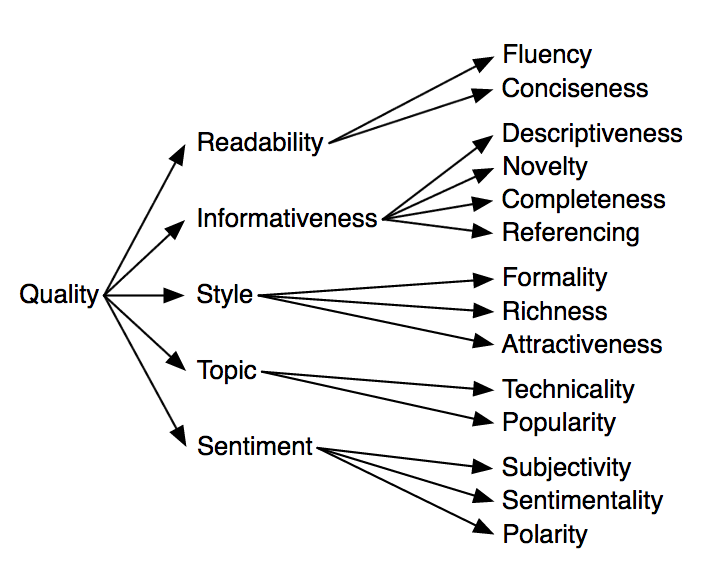
\includegraphics[scale=0.6]{Dimensions.png}
\end{center}

\indent Their approach, however, is not as effective as it could be because it assumes that writers are incompetent and editors are trying to maintain high article quality.  Our group believes this project is best approached like a security problem whether the writer is analogous to a malicious attacker, where a model or system would be used defensively by the consumer to protect against malicious news feeds. \\
\indent This assumption appears to have merit as BuzzFeed conducted an extensive study regarding articles published by highly partisan Facebook pages (e.g. 'Eagle Rising' and 'Occupy Democrats').  The results indicate that partisan pages are much more widely shared and had significant less veracity than mainstream articles.

\begin{center}
	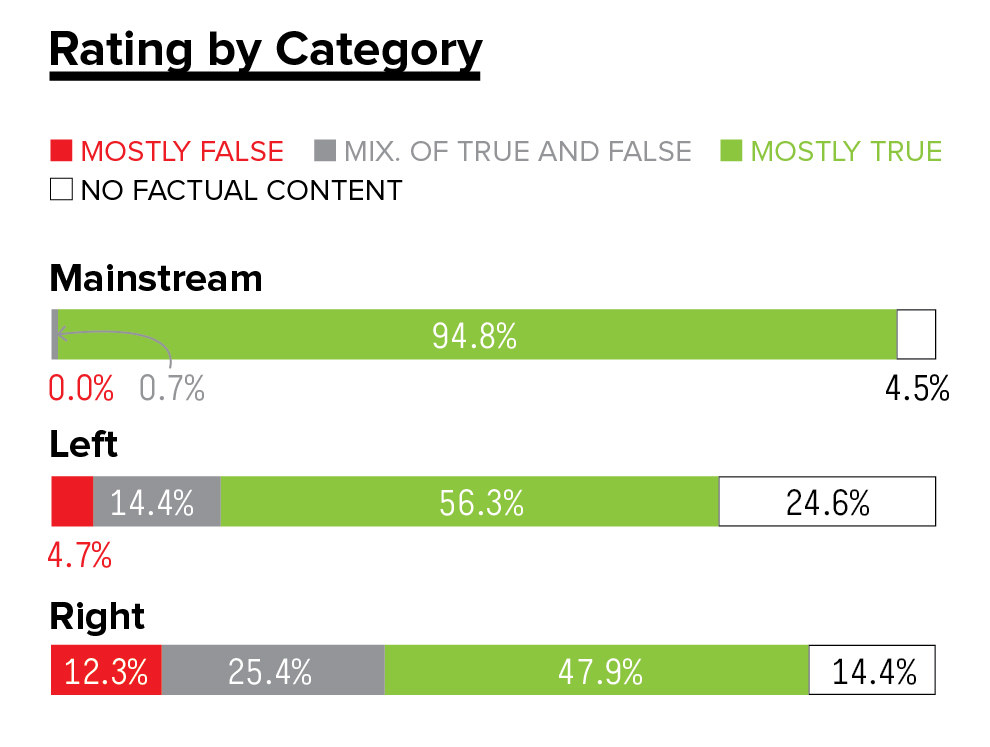
\includegraphics[scale=0.2]{BuzzFeedRatings.jpg}
\end{center}

\begin{center}
	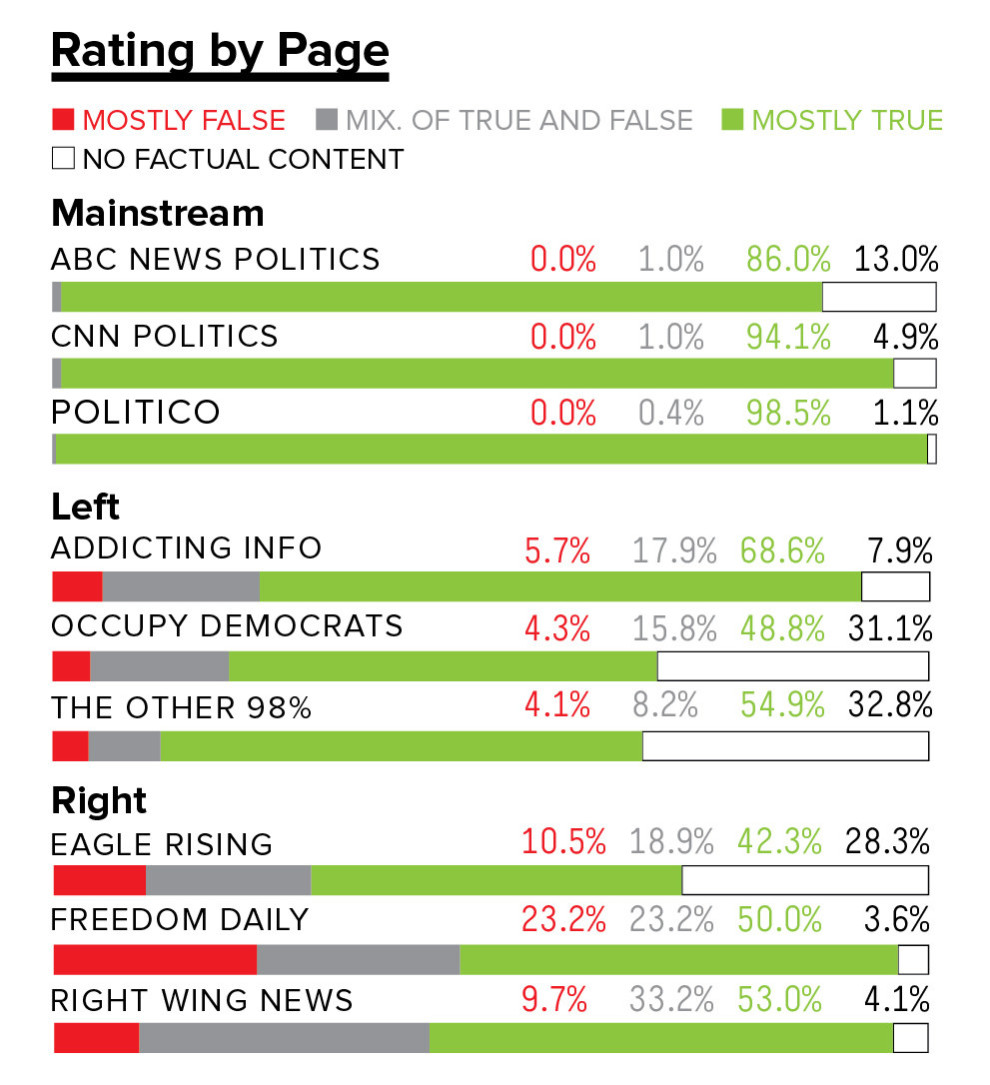
\includegraphics[scale=0.2]{PageVeracity.jpg}
\end{center}

\begin{center}
	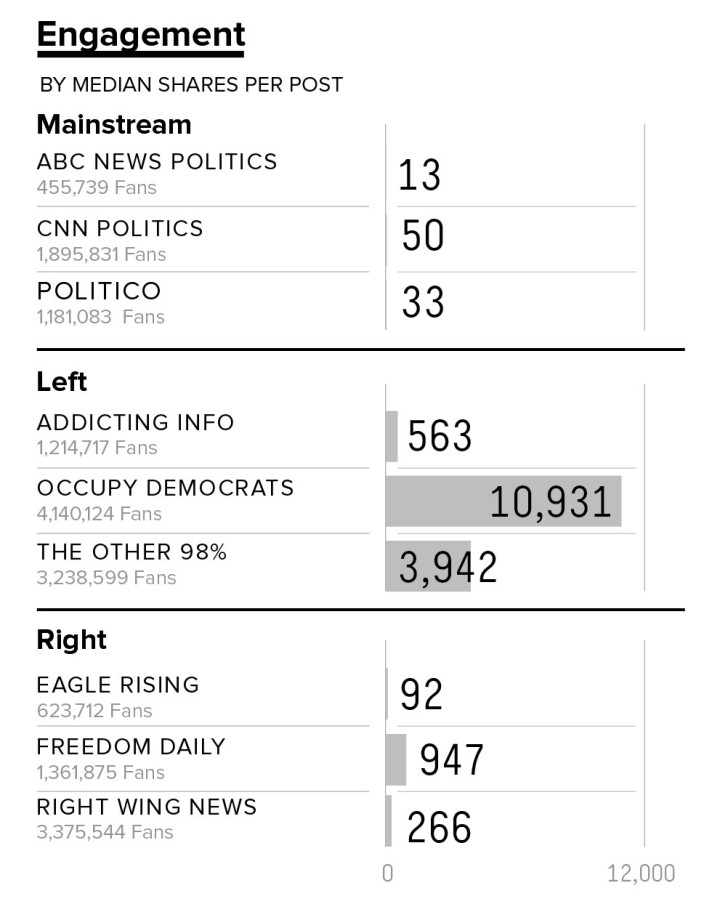
\includegraphics[scale=0.2]{Engagement.jpg}
\end{center}

\indent Therein lies the crux of the problem, and our project aims to alleviate the scope and impact of misinformation campaigns.

\section{Methods and Results}

\indent \indent We established a benchmark using Kim Yoon’s CNN for Sentence Classification. This is a popular benchmarking approach for text classification. We first process the dataset into input X (article full content) and input Y (two dimensional array, one-hot encoded for article quality) and feed the dataset to the model for training. \\
\indent The CNN model consists of several layers. First layer embeds words in article content into low-dimensional vectors. The second layer performs convolutions over the embedded word vectors using multiple filter sizes. At the end, we max-pool the result of the convolutional layer into a long feature vector, added dropout regularization and classify the result using a softmax layer.  Table 1 shows our initial results on all 14 aspects of news quality. The last row shows the overall quality classification result.

\begin{table}[h]
\begin{center}
\begin{tabular}{|l|rl|}
\hline \bf Type & \bf Evaluation Acc & \bf Best Train Acc \\ \hline
Formality & 0.830769 & 0.84 \\
Fluency & 0.676923 & 0.7 \\
Conciseness & 0.630769 & 0.64 \\
Descriptiveness' & 0.769231 & 0.771739 \\
Novelty& 0.815385 & 0.815385 \\
Completeness & 0.676923  & 0.77\\
Referencing & 0.8 & 0.8 \\
Richness & 0.846154 & 0.846154 \\
Attractiveness & 0.892308 & 0.91 \\
Technicality & 0.861538 & 0.89 \\
Popularity & 0.861538 & 0.87 \\
Subjectivity & 0.923077 & 0.99 \\
Positive Emotion & 0.969231 & 0.99 \\
Negative Emotion & 0.969231 & 0.969231 \\
 &  &  \\
Quality & 0.846154 & 0.846154 \\
\hline
\end{tabular}
\end{center}
\caption{\label{font-table} News quality classification results on different aspects. }
\end{table}

\indent After benchmarking, we trained fourteen separate CNNs with an 80/20 train-dev split with 6-fold validation.  The purpose was to look for correlations between the article quality features and article veracity on the BuzzFeed article veracity dataset.  By using the trained quality dimension models to predict the BuzzFeed article quality attributes, we could then see if certain attributes were more present in truthful articles as opposed to untruthful ones.\\
\indent The process involved manually extracting article text from the BuzzFeed Facebook article links with somewhat-balanced representation for all of the categories.  We ended up with 159 articles ranging from 'Mostly True' to 'Mostly False' that were hand labeled by BuzzFeed's dataset creators.
\indent We then passed the BuzzFeed articles to each of the trained CNNs to see what the model accuracy / correlation was when predicting veracity given a model trained on a specific dimension of quality.

\section{Results}

\indent \indent The results on the training and test data look quite good for predicting the fourteen different dimensions:
\begin{center}
	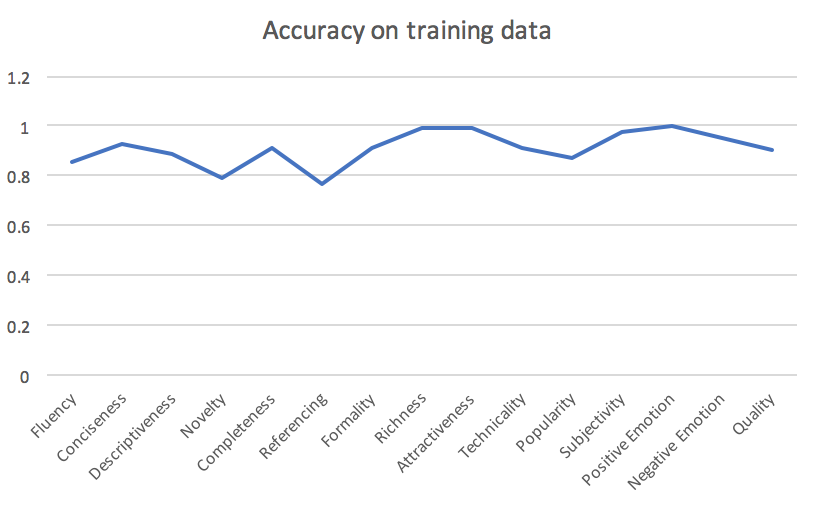
\includegraphics[scale=0.5]{Training.png}
\end{center}

The results seem poor, however, when extending the Article Quality models to the Facebook BuzzFeed dataset to look for correlation between a quality dimension and the veracity of an article.  It appears fair to say, however, that the results are inconclusive at the moment due to lack of data and because other options exist to possibly make a working and useful model to connect quality and veracity.
\begin{center}
	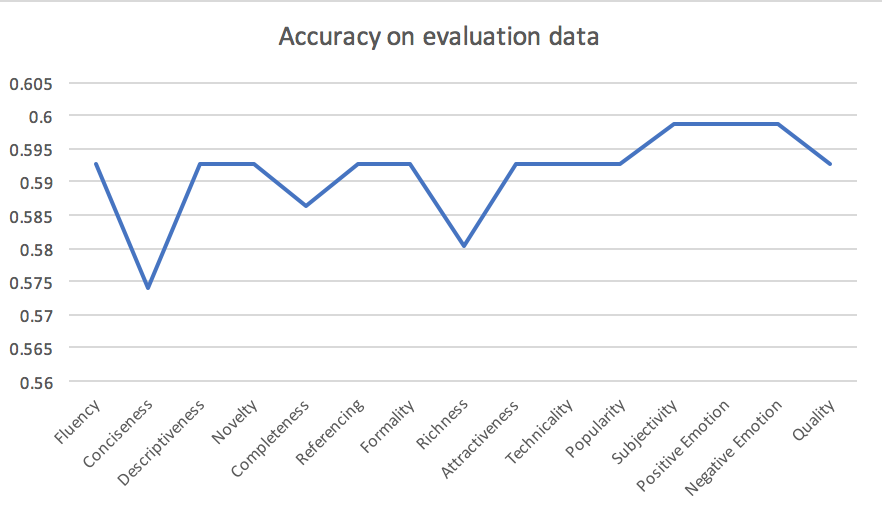
\includegraphics[scale=0.5]{Results.png}
\end{center}

\section{Conclusion}

\indent \indent It is definitely possible to label articles accurately based upon the fourteen dimensions of quality discussed in this paper, and there may be some merit in using article quality in conjunction with the article content to automatically judge article veracity.  This evidence is mostly anecdotal, however, based upon our experience sifting through the BuzzFeed Facebook articles--there was a clear writing style and choice of diction associated with untruthful articles.\\
\indent Unfortunately, we ran out of time and did not get to a working ensemble model to accurately judge veracity as we envisioned, but we believe further work on this can and will bear fruit.  The next best course of action is to properly create and curate sufficient high-quality content to evaluate the connection between quality and veracity with the working Article Quality model and then build a working ensemble that consumes the article content (e.g. text, website, etc) along with the set of quality features (e.g. conciseness) to create an accurate predict on veracity ('Mostly True' or 'Not Mostly True').


\section*{Acknowledgments}

\indent \indent Thanks to Joao Magalhaes, Ioannis Arapakis etc. who kindly helped us understanding their publication and helped us finding their dataset online. Also thanks to Denny Britz, who kindly shared his text classification approach using Convolutional Neural Network. His methods have been widely used for model benchmark, and helped us to set a decent start point of our research. 

\section*{References }

\begin{enumerate}
	\item \url{http://fortune.com/2017/04/05/ebay-pierre-omidyar-100m-fight-fake-news/} 
	\item \url{http://bigstory.ap.org/article/d5b1763ae5ad463ba8bc4fff5fa23816/9-eu-nato-nations-set-center-fight-hybrid-threats}
	\item \url{http://www.snopes.com/obama-signs-christmas-bill-making-alternative-media-illegal/} 
	\item \url{http://www.cnbc.com/2017/04/27/facebook-to-fight-fake-news-groups.html}
	\item \url{https://github.com/BuzzFeedNews/2016-10-facebook-fact-check}
	\item \url{http://aclweb.org/anthology/P/P16/P16-1178.pdf}
	\item \url{https://www.researchgate.net/profile/Victoria_Rubin/publication/281818851_Deception_Detection_for_News_Three_Types_of_Fakes/links/55f96a9b08aeafc8ac24260e.pdf}
	\item \url{https://pdfs.semanticscholar.org/b112/1655f0858ba38226a4dd614e84cb86c2a8a6.pdf}
	\item \url{http://ethesis.nitrkl.ac.in/3578/1/thesis.pdf}
	\item \url{http://www.aclweb.org/anthology/W/W16/W16-0802.pdf}
	\item \url{http://www.journalism.org/2016/07/07/pathways-to-news/ }
	\item \url{https://www.kaggle.com/mrisdal/fake-news}
	\item \url{http://novasearch.org/datasets/ }
	\item \url{http://www.wildml.com/2015/12/implementing-a-cnn-for-text-classification-in-tensorflow/ }
\end{enumerate}

\end{document}
